\chapter{System Configuration}\label{sec:system-configuration}

\section{SCION Switch}
A SCION switch connects all SCION elements within an \AD to abstract intra-\AD communication. SCION defines a new inter-\AD routing architecture (including corresponding protocols), yet does not mandate any intra-\AD architecture. Hence, an \AD will be able to adopt SCION without changing the current internal forwarding/routing mechanisms. A SCION switch is a special element that virtualizes intra-\AD communication and can be replaced by intra-\AD forwarding/routing mechanisms in real operation.

All SCION elements such servers and border routers are assigned a unique AID and should be reached with their AID. A SCION switch simply maintains its port to an element's AID mapping to enables communication between elements. AID = 0xFFFFFFFFFFFFFFFF is reserved for broadcasting a message to all elements; e.g., server list announcement. A SCION switch constructs a map between an output port and the AID of the connected element to the port during initialization. Specifically, a SCION switch sends AID request messages (AID\_REQ) to all output ports and the connected elements reply with their own AID (AID\_REP). The SCION switch constructs a AID-to-port mapping table using the AID reply arrived at each port. Note that an input port does not need to be mapped to the connected element's AID since a switch does not write (and hence route) any packet to the port (i.e., read-only port).

\begin{figure}[ht]
\centering
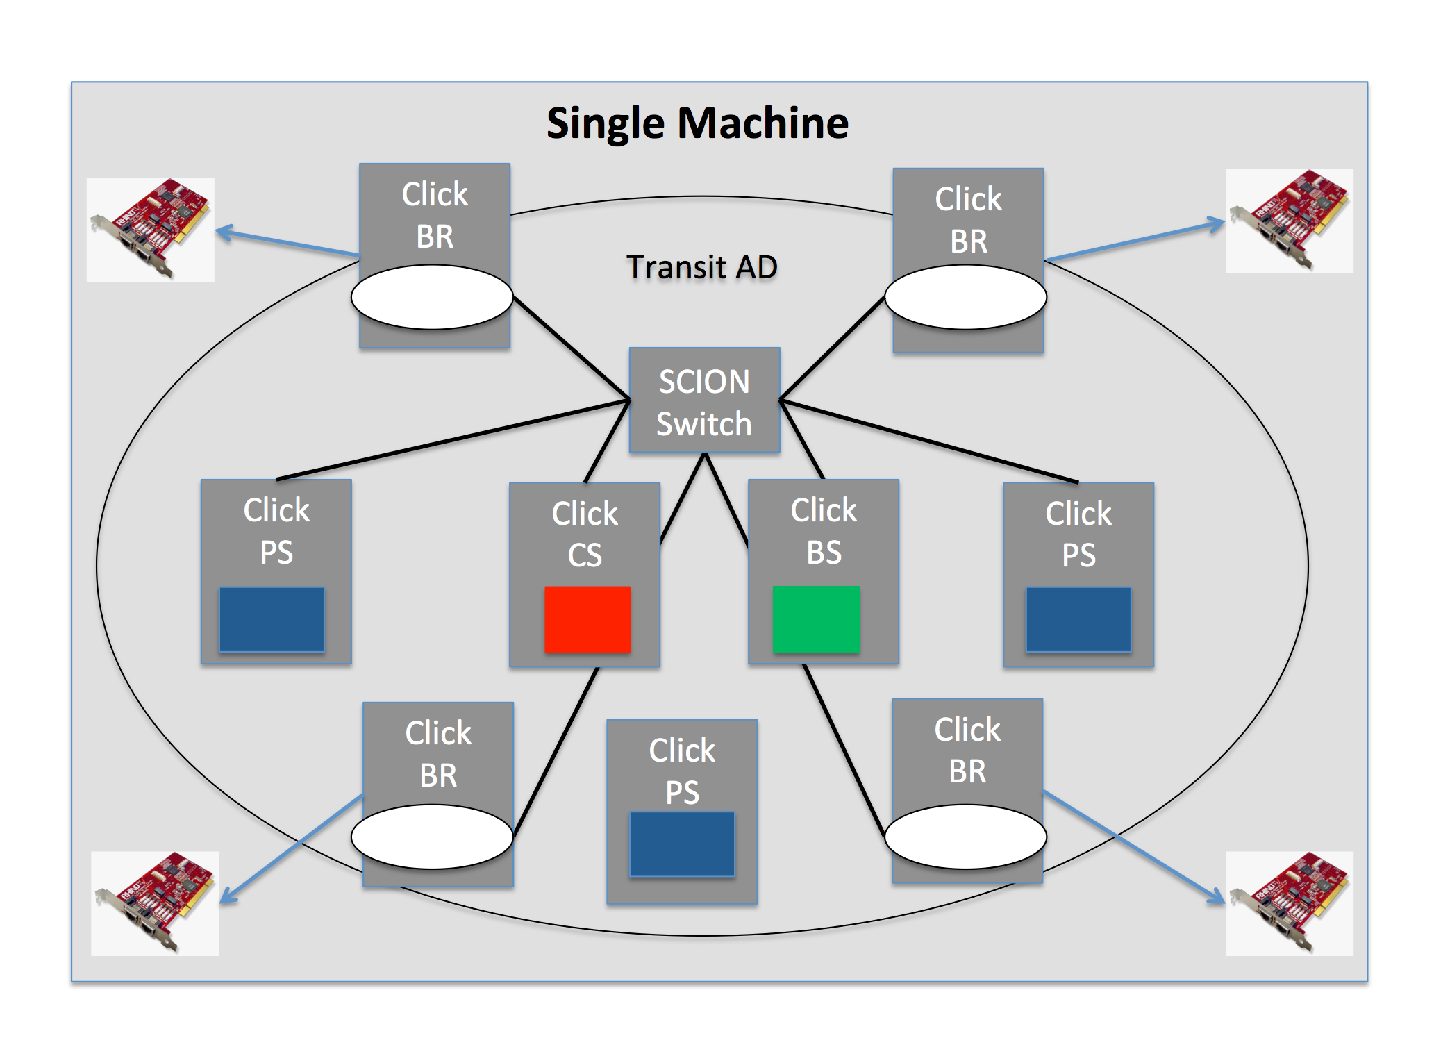
\includegraphics[width=.8\columnwidth]{./fig/configuration.eps}
\caption{Configuration. All elements are connected through a SCION switch.\newline
BR: Border Router, CS: Certificate Server, BS: Beacon Server, PS: Path Server}\label{fig:configuration}
\end{figure}

Figure~\ref{fig:configuration} illustrates how elements are interconnected through a SCION switch within an \AD. In this example, border routers connect to other \ADs through an NIC. Yet, multiple \ADs can be configured in a single machine or each \AD can be configured in a separate virtual machine.


\section{Click Configuration File}
Currently, we have five types of Click elements, which are Certificate Server, Beacon Server, Path Server, Border Router and SCION Switch.  
Each element is configured in a .click file (i.e., a click router configuration file) as follows.

Note: every element has its own (object) name for .click file generation. This name is meaningful in .click file.

\begin{itemize}
\item Certificate Server: AID, Address Type, Address, Configuration File, Topology File, RoT File.
\item Beacon Server: AID, Address Type, Address, Configuration File, Topology File, RoT File.
\item Path Server:AID, Address Type, Address, Configuration File, Topology File.
\item Border Router:AID, Address Type, Address, Configuration File, Topology File.
\item SCION Switch:
\end{itemize}

\section{SCION Configuration File}
In addition to the basic configuration parameters, more detailed parameters specific to each element are defined in .conf file. In other words, each element has its own configuration file and intializes itself with this file. The configuartion paratmers of individual elements are shown below.

\begin{itemize}
\item Certificate Server: ADID, ISDID, RegTime, PropTime, Log Level, Private Key File, Certificate File, Master OFG Key, Master AD Key.
\item Beacon Server: ADID, ISDID, RegTime, PropTime, Log Level, Private Key File, Certificate File, Master OFG Key, Master AD Key, PCB Queue Size, Number of Registered Path, Number of Up Path, Register Path (bool).
\item Path Server: Path Server Queue Size,  Log File.
\item Border Router: Queue Size, Log File, Interfaces, Master OFG Key, Master AD Key. 
\item SCION Switch:
\end{itemize}


\begin{comment}
\section{Interconnect}
\begin{itemize}
\item Intra-machine
\item Inter-machine
\end{itemize}
\end{comment}

